\section{Phases and reconstruction}\label{sec:partII-H}

We prove the phase decomposition of Theorem~\ref{prop:PH} and the reconstruction of Theorem~\ref{prop:RC}, starting from the correlations of Theorem~\ref{prop:IV}, the quotient fields of Proposition~\ref{prop:FC}, the slab operators of Lemma~\ref{lem:H1.1}, the rotations of Lemma~\ref{lem:G3.1} and the tensor of Theorem~\ref{prop:ST}. Three different objects appear, and only the first two are used here.
\begin{center}
\small
\begin{tabular}{p{0.36\textwidth}p{0.55\textwidth}}
\toprule
object & role\\
\midrule
separated correlations $S^\xi_n$ of a phase & Euclidean correlations, with reflection positivity on positive-time words (Section~\ref{sec:partII-H.1})\\
ordered-time continuations $\mathsf F^\xi_n$ and boundary distributions $W^\xi_n$ & construction of the tempered Wightman functions and the relativistic fields (Section~\ref{sec:partII-H.2})\\
contact extensions of Theorem~\ref{prop:CT} & a specified Euclidean extension through collisions with controlled local order (Section~\ref{sec:partII-J}); not used in the reconstruction\\
\bottomrule
\end{tabular}
\end{center}
The reconstruction thus proceeds from separated Euclidean correlations and slab bounds; it does not require a positive Euclidean extension across collision diagonals.

We keep the words, reflections $\vartheta,\theta$, insertion rule and slab operators $\mathsf B_h(w)$ of Section~\ref{sec:G-coordinate}.

\subsection{Compression and phases}\label{sec:partII-H.1}

Put $P_0=P_4^0$ and $\Omega=\Omega_4^{\rm OS}$ in this subsection, and write $U_y$, $y^4=0$, for spatial translations on the OS space. Compression does the following. A long empty time interval removes the positive-energy components: $\mathsf B_{h+t}(w)=\mathsf B_h(w)e^{-tH_4^{\rm OS}}$ and $e^{-tH_4^{\rm OS}}\to P_0$. The surviving insertions $M^0(w)=P_0\mathsf B_h(w)|_{\ker H_4^{\rm OS}}$ commute (Lemma~\ref{lem:H1.2}), and a character of the algebra they generate assigns a compatible scalar to every compressed insertion; integrating over characters against the vacuum state gives the mixture formula. A phase is such a character, not a set of field configurations. Commutativity alone does not show that each character is reflection invariant, or that no field direction is lost in it: a lattice variance inequality gives the first, and the chessboard inequality preserves the rank of finite families of field tests (Lemma~\ref{lem:H1.3}). Figure~\ref{fig:H-spaces} shows where each of these objects lives.

\begin{figure}[t]
\centering
\begin{tikzpicture}[font=\small,>={Stealth[length=2mm]}]
\node (H) at (0,0) {$\mathcal H_4^{\rm OS}$};
\node (K) at (4.4,0) {$\ker H_4^{\rm OS}\ni\Omega$};
\node (A) at (8.4,0) {$\mathfrak A_0$};
\node[below=1pt of A,font=\footnotesize] (Ag) {generated by $M^0(w)=P_0Y_w$};
\node (C) at (11.6,0) {$\C$};
\draw[->] (K) to[bend right=22] node[above] {$Y_w$} (H);
\draw[->] (H) to[bend right=22] node[below] {$P_0$} (K);
\draw[->] (A) -- node[above] {acts on} (K);
\draw[->] (A) -- node[above] {$\xi\in\phases$} (C);
\node (Hx) at (4.4,-2.4) {$\mathcal H_{4,\xi}^{\rm OS}$};
\node (Hw) at (0,-2.4) {$\mathcal H_\xi$};
\draw[->] (Hw) -- node[above] {$\mathsf J_\xi^{\rm OS}$} node[below] {unitary} (Hx);
\draw[->] (Ag.south) |- node[pos=0.75,below] {$\langle[v]_\xi,[w]_\xi\rangle=\xi(Y_v^*Y_w)$} (Hx);
\end{tikzpicture}
\caption{The spaces and maps of this section. A positive word~$w$ in a slab gives the insertion $Y_w$ from the full ground space $\ker H_4^{\rm OS}$ of the mixture, which need not be a line, into its OS space; compression by the ground projection~$P_0$ gives~$M^0(w)$, and these operators generate the commutative algebra~$\mathfrak A_0$. A phase is a character~$\xi$ of~$\mathfrak A_0$. The OS space of the phase is the completion of positive words under the form $\xi(Y_v^*Y_w)$, the value of~$\xi$ on the compression of a whole word, which need not be the product of the values on its two halves~\eqref{eq:H-compression-defect}. Its ground space is a line for $\nu$-almost every phase by Lemma~\ref{lem:H1.3} and for every phase by Lemma~\ref{lem:H2.3}. The relativistic space~$\mathcal H_\xi$ of Section~\ref{sec:partII-H.2} is identified with it by the unitary map of Lemma~\ref{lem:H2.2}.}
\label{fig:H-spaces}
\end{figure}

\begin{figure}[t]
\centering
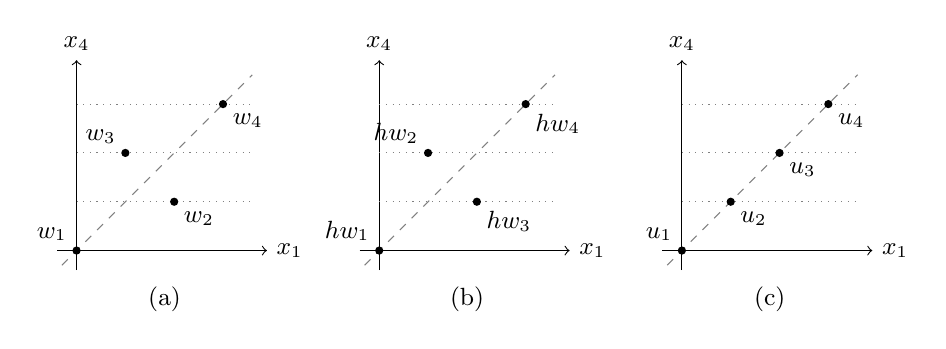
\begin{tikzpicture}[scale=0.62,font=\small]
\foreach \dx/\tag in {0/(a),6.2/(b),12.4/(c)}{
  \begin{scope}[xshift=\dx cm]
  \draw[->] (-0.4,0) -- (3.9,0) node[right] {$x_1$};
  \draw[->] (0,-0.4) -- (0,3.9) node[above] {$x_4$};
  \draw[dashed,gray] (-0.3,-0.3) -- (3.6,3.6);
  \foreach \t in {1,2,3}{\draw[dotted,gray] (0,\t) -- (3.6,\t);}
  \node at (1.8,-1.0) {\tag};
  \end{scope}}
\foreach \p/\l/\a in {(0,0)/w_1/above left,(2,1)/w_2/below right,(1,2)/w_3/above left,(3,3)/w_4/below right}{
  \fill \p circle (2.4pt) node[\a] {$\l$};}
\begin{scope}[xshift=6.2cm]
\foreach \p/\l/\a in {(0,0)/hw_1/above left,(2,1)/hw_3/below right,(1,2)/hw_2/above left,(3,3)/hw_4/below right}{
  \fill \p circle (2.4pt) node[\a] {$\l$};}
\end{scope}
\begin{scope}[xshift=12.4cm]
\foreach \k in {0,1,2,3}{\fill (\k,\k) circle (2.4pt);}
\node[above left] at (0,0) {$u_1$}; \node[below right] at (1,1) {$u_2$};
\node[below right] at (2,2) {$u_3$}; \node[below right] at (3,3) {$u_4$};
\end{scope}
\end{tikzpicture}
\caption{The axis exchange in the proof of Lemma~\ref{lem:H1.2}, in the plane of the first and fourth coordinates, in units of~$j$; time~$x_4$ is vertical, and the dashed line is fixed by the exchange~$h$. (a)~Four words, in time order $w_1,w_2,w_3,w_4$. (b)~After~$h$ the set of points is the same, but the transformed middle words have traded places, so the time order is $hw_1,hw_3,hw_2,hw_4$. (c)~On the diagonal, $h$ moves no point and changes no time order; this identity removes~$h$ from the products.}
\label{fig:H-exchange}
\end{figure}

Rotations make spatial translations trivial at zero energy; compression then removes slab width and placement.
\begin{lemma}[Compression algebra]\label{lem:H1.2}
The operators $M^0(w)$ are independent of the slab width and placement. They generate a separable commutative unital C$^*$-algebra~$\mathfrak A_0$ on $\ker H_4^{\rm OS}$, with cyclic and separating vector~$\Omega$. Its character space~$\phases$ is compact metric, the vacuum state is given by a full-support probability measure~$\nu$, and
\begin{equation*}
S^\xi(w)=\xi(M^0(w)),\qquad S(w)=\int_{\phases}\xi(M^0(w))\,d\nu(\xi)\,.
\end{equation*}
\end{lemma}
\begin{proof}
For fixed words and large~$z^4$ the correlation is $\langle v,U_{\vec z}e^{-(z^4-c)H_4^{\rm OS}}v'\rangle$, and strong heat convergence makes fixed time shifts negligible, uniformly in~$\vec z$. Choose an orthogonal reflection~$K$ taking $y+e_4$ to $|y+e_4|e_4$. Since $\langle K(y+e_4),Ke_4\rangle=1$, the ray $tKe_4$ has positive time component. By the covariance of Lemma~\ref{lem:G3.1}, rotating the displacements $te_4+y+e_4$ and~$te_4$ makes their difference purely temporal, so their correlations become equal in the limit; removing the extra~$e_4$ gives $U_yP_0=P_0$ by density.

The identities $\mathsf B_{h+t}(w)=\mathsf B_h(w)e^{-tH_4^{\rm OS}}$ and $\mathsf B_{h+t}(\tau_{te_4}w)=e^{-tH_4^{\rm OS}}\mathsf B_h(w)$ give width and placement independence of $M^0(w)$, and $M^0(w)\Omega=P_0[w]$, $\langle\Omega,M^0(w)\Omega\rangle=S(w)$. Successive use of~\eqref{eq:H-slab-laws} proves the cluster identity
\begin{equation}\label{eq:H-clusters}
\lim_{j\to\infty}S\bigl(\tau_{z_1(j)}w_1\cdots\tau_{z_m(j)}w_m\bigr)
=\langle\Omega,M^0(w_1)\cdots M^0(w_m)\Omega\rangle
\end{equation}
whenever $(z_{i+1}(j)-z_i(j))^4\to\infty$; in the induction, $\psi_j\to\psi$ and $t_j\to\infty$ imply $U_{y_j}e^{-t_jH_4^{\rm OS}}\psi_j\to P_0\psi$ for arbitrary~$y_j$.

\emph{Commutativity.} Let $h\in O(4)$ exchange the first and fourth coordinates, and write $hw$ for the word whose points, internal offsets included, and labels are transformed by~$h$, the labels through the representations of Lemma~\ref{lem:G3.1}. Place four words $w_1,\ldots,w_4$ at
\begin{equation*}
z_1=0,\quad z_2=j(e_4+2e_1),\quad z_3=j(2e_4+e_1),\quad z_4=3j(e_4+e_1),
\end{equation*}
with times $0,j,2j,3j$ (Figure~\ref{fig:H-exchange}). The points $hz_i$ have times $0,2j,j,3j$: the two middle words exchange their time order. Covariance and~\eqref{eq:H-clusters}, applied before and after~$h$, give
\begin{equation*}
\langle\Omega,M^0(w_1)M^0(w_2)M^0(w_3)M^0(w_4)\Omega\rangle
=\langle\Omega,M^0(hw_1)M^0(hw_3)M^0(hw_2)M^0(hw_4)\Omega\rangle .
\end{equation*}
The right side still carries~$h$. Words $u_k$ at the points $(k-1)j(e_4+e_1)$, $k=1,\ldots,4$, which $h$ fixes, keep their time order, so the same two identities give $\langle\Omega,\prod_kM^0(hu_k)\Omega\rangle=\langle\Omega,\prod_kM^0(u_k)\Omega\rangle$. With $(u_k)=(w_1,w_3,w_2,w_4)$ this removes~$h$:
\begin{equation*}
\langle\Omega,M^0(w_1)\bigl[M^0(w_2),M^0(w_3)\bigr]M^0(w_4)\Omega\rangle=0 .
\end{equation*}
The vectors $M^0(w_4)\Omega=P_0[w_4]$ span a dense subspace of $\ker H_4^{\rm OS}$. By~\eqref{eq:H-slab-laws}, the reflection $w_1=\theta v$ of a positive word~$v$ has $M^0(w_1)=M^0(v)^*$, so the vectors $M^0(w_1)^*\Omega=P_0[v]$ do too. Hence $M^0(w_2)$ and $M^0(w_3)$ commute. Density also gives cyclicity, and the empty word gives the unit. If $a\Omega=0$, then $ab\Omega=0$ on this span, so $a=0$. Basis labels and countable dense position sets generate~$\mathfrak A_0$ by norm continuity. Gelfand theory and the vacuum state give the compact metric spectrum and the probability measure~\cite[Theorems~2.4.1 and~2.8.2]{Landsman1998}; separation gives full support, since $\int|\xi(a)|^2d\nu=\|a\Omega\|^2$ vanishes only for $a=0$.
\end{proof}

Compression does not preserve products, and the identities used below have separate jobs. For a positive word~$v$ in a slab of width~$h$ put $Y_v=\mathsf B_h(v)|_{\ker H_4^{\rm OS}}$, a bounded map from $\ker H_4^{\rm OS}$ to~$\mathcal H_4^{\rm OS}$. Then $M^0(v)=P_0Y_v$, and~\eqref{eq:H-slab-laws} gives $M^0(\theta v\,w)=Y_v^*Y_w$ for the reflected whole word. For bounded operators $A,B$ and an orthogonal projection~$P_0$ one has $P_0ABP_0-(P_0AP_0)(P_0BP_0)=P_0A(1-P_0)BP_0$; here it reads
\begin{equation}\label{eq:H-compression-defect}
M^0(\theta v\,w)-M^0(v)^*M^0(w)=Y_v^*(1-P_0)Y_w\,.
\end{equation}
A character is multiplicative on~$\mathfrak A_0$, but a phase evaluates a word at finite separation through the compression of the whole word, $S^\xi(\theta v\,w)=\xi(Y_v^*Y_w)$. In the OS space of the phase, $\xi(M^0(v)^*M^0(w))=\langle[v]_\xi,\Omega_\xi^{\rm OS}\rangle\langle\Omega_\xi^{\rm OS},[w]_\xi\rangle$, so the character of the right side of~\eqref{eq:H-compression-defect} is the part of $\langle[v]_\xi,[w]_\xi\rangle$ orthogonal to the phase vacuum; it vanishes for all~$v,w$ only if that space is the line~$\C\Omega_\xi^{\rm OS}$. A long empty time interval between the two halves replaces $1-P_0$ by $e^{-tH_4^{\rm OS}}-P_0$, which tends to zero strongly. This is the mechanism of the cluster identity~\eqref{eq:H-clusters}, which produces products and hence commutativity; the whole-word identity $M^0(\theta v\,w)=Y_v^*Y_w$ produces the positivity of the phase OS form in Lemma~\ref{lem:H1.3}.

Moment bounds in the vacuum state bound a compressed operator in every phase. This is the form in which lattice chessboard estimates enter here and in Sections~\ref{sec:partII-I}--\ref{sec:partII-J}.
\begin{lemma}[Vacuum moments bound compressed operators]\label{lem:H-roots}
Let $U\in\mathfrak A_0$ and $B\ge0$ satisfy $\langle\Omega,(U^*U)^n\Omega\rangle\le B^{2n}$ for every $n\in\N$. Then $\|U\|=\sup_{\xi\in\phases}|\xi(U)|\le B$.
\end{lemma}
\begin{proof}
By Lemma~\ref{lem:H1.2}, $\langle\Omega,(U^*U)^n\Omega\rangle=\int|\xi(U)|^{2n}\,d\nu(\xi)$. If $|\xi_0(U)|>b>B$, continuity gives an open neighbourhood~$O$ of~$\xi_0$ on which $|\xi(U)|>b$, and full support gives $\nu(O)>0$. Then $\nu(O)b^{2n}\le B^{2n}$ for every~$n$, which is impossible. Gelfand theory identifies $\|U\|$ with $\sup_\xi|\xi(U)|$.
\end{proof}
The moment hypothesis comes from the lattice as follows. Let a lattice word difference be interior with centered chessboard seminorm at most~$B_0$ in one cell, multiplied by exterior insertions with centered chessboard seminorms at most $B_1,\ldots,B_L$ in disjoint finer cells, and let $U\in\mathfrak A_0$ be its compressed limit along the ordered limit. Apply~\eqref{eq:F-chess} to $2n$ widely translated copies, alternately conjugated; take the ordered limits and then infinite translation separation, using~\eqref{eq:H-clusters}; reflection identifies the alternating copies with adjoints. This gives $\langle\Omega,(U^*U)^n\Omega\rangle\le(B_0\prod_lB_l)^{2n}$, hence $\|U\|\le B_0\prod_lB_l$.

A generic grid word has positions in $a_k\Z^4$ with pairwise distinct coordinates along each axis. For real coefficient representatives~$(d_i,c_i)$ write $\langle\cdot\rangle_{N,p}$ for the Wilson expectation of Section~\ref{sec:wilson}, and put $\mathcal O_{N,p}(w)=\prod_i O^{(d_i)}_{N,p}(c_i,x_i/a_N)$. The word differences used below are
\begin{equation}\label{eq:H-real-approx}
f_{j,N,p,T}=\mathcal O_{N,p}(\tau_{z_j(T)}w)-\mathcal O_{N,p}(\tau_{z_j(T)}\vartheta w),\qquad z_j(T)=Tja_k(1,1,1,1).
\end{equation}
For each degree bound and lower grid level~$m$, Lemma~\ref{lem:E2-bounded-real} chooses $k\ge m$ before~$w$; these are the cofinal grids used below. For $\varepsilon>0$ it supplies real $g_{j,N,p,T}$ and a finite $R_\varepsilon$, independent of $N,p,T,j$, with $|g_{j,N,p,T}|\le R_\varepsilon$ eventually in the ordered cutoffs for each fixed~$T,j$, and, for $i<j$ and large~$T$, eventually in the ordered cutoffs, $|\langle g_ig_j\rangle_{N,p}-\operatorname{Re}\langle f_if_j\rangle_{N,p}|\le\varepsilon$; the threshold may depend on $T,i,j$. Bounded~$g_i$ control the diagonal variance terms, for which $f_i^2$ has no uniform bound.

\begin{lemma}[Phase fields and selection]\label{lem:H1.3}
For every $\xi\in\phases$, its table satisfies E1--E7, retains the inclusions, derivatives, conjugation, rotations and stress identities of the mixture, and
\begin{equation*}
\nullspace{d}(S^\xi)=\nullspace{d}(S)\qquad(d\in\N)\,.
\end{equation*}
Each separated value is continuous in~$\xi$. For $\nu$-almost every~$\xi$, the time-axis OS ground space is one-dimensional.
\end{lemma}
\begin{proof}
\emph{Reflection and rotation invariance.} We first prove
\begin{equation}\label{eq:H-reflection}
M^0(\vartheta w)=M^0(w),\qquad M^0(hw)=M^0(w)\quad(h\in O(4))\,.
\end{equation}
For a real grid word set $Z=M^0(w)-M^0(\vartheta w)$. Equation~\eqref{eq:H-slab-laws} gives $Z^*=-Z$, so $a=\langle\Omega,Z^2\Omega\rangle=-\|Z\Omega\|^2\le0$. Lattice variance gives
\begin{equation*}
0\le\left\langle\left(\sum_{i=0}^qg_i\right)^2\right\rangle
\le(q+1)R_\varepsilon^2+2\sum_{i<j}\left(\operatorname{Re}\langle f_if_j\rangle+\varepsilon\right)\,.
\end{equation*}
For fixed $q,T$, intersect the finitely many eventual sets, take the ordered cutoffs, then $T\to\infty$. Each pair expands into four separated moments, whose signed sum tends to~$a$ by Lemma~\ref{lem:E3.1}, \eqref{eq:F-conf} and~\eqref{eq:H-clusters}. Thus $0\le(q+1)[R_\varepsilon^2+q(a+\varepsilon)]$; first $q\to\infty$, then $\varepsilon\downarrow0$, gives $a\ge0$, and separation of~$\Omega$ gives $Z=0$. Grid density, norm continuity and multilinearity give all words. For the second identity, the cluster identity gives simultaneous orthogonal invariance of two-factor vacuum entries along rays with positive time before and after rotation; such a ray exists unless time is reversed, when composition with~$\vartheta$ suffices. With $v=M^0(u)\Omega$ and $x=M^0(w)\Omega$, simultaneous invariance and time-reflection invariance give $\langle v,x\rangle=\langle g^{-1}v,\vartheta g^{-1}x\rangle=\langle v,g\vartheta g^{-1}x\rangle$. Density gives every hyperplane reflection, and an orthogonal map is a product of at most four reflections.

\emph{Euclidean properties.} Testing on positive words gives the permutation, unit and linearity identities and annihilates mixed null labels, so $\nullspace{d}(S)\subset\nullspace{d}(S^\xi)$. Character evaluation gives reality, covariance and smooth phase values, continuous in~$\xi$. For positive words~$w_i$ in a common slab write $Y_i=Y_{w_i}\colon\ker H_4^{\rm OS}\to\mathcal H_4^{\rm OS}$. Since $M^0(\theta w_iw_j)=Y_i^*Y_j$,
\begin{equation*}
\sum_{i,j}\bar c_ic_jM^0(\theta w_iw_j)=\left(\sum_i c_iY_i\right)^*\left(\sum_jc_jY_j\right)\ge0\,.
\end{equation*}
The entries are compressions of whole words, not the products $M^0(w_i)^*M^0(w_j)$ (see~\eqref{eq:H-compression-defect}); a character applied to them gives a positive semidefinite matrix, which need not have rank one. Spectral permanence and character evaluation preserve positivity~\cite[Theorems~2.5.1(1) and~2.6.4]{Landsman1998}, and coordinate rotations give every axis; integrating the vectors of this positive Gram kernel against compact positive-time joint tests expresses the smeared OS form as a norm square. Inclusions and derivatives pass through bounded compression and character evaluation. To transfer the shell identities, extend the character $\xi$ by the complex Hahn--Banach theorem to a bounded linear functional $\widetilde\xi$ on $\mathcal B(\ker H_4^{\rm OS})$, and put
\[
 \ell_\xi(T)=\widetilde\xi(P_0T|_{\ker H_4^{\rm OS}}),
 \qquad T\in\mathcal B(\mathcal H_4^{\rm OS}).
\]
This is a fixed bounded linear functional; no positivity or multiplicativity of its extension is needed. On a slab insertion it evaluates the compressed whole word and hence gives $S^\xi$.

Fix a distinguished insertion, finitely many distinct spectators and an admissible smooth compactly supported shell cutoff $\chi$, equal to one near the distinguished point and supported away from the spectators. Translate the entire configuration and $\operatorname{supp}\chi$ into one slab with positive boundary margins. For each shell weight $q(y)$ occurring in Theorem~\ref{prop:ST}, including the linear rotational factor, multiply the slab operator with the stress inserted at $y$ by $q(y)$. The weight has compact support away from every insertion. Set the product to zero near the collision points; by the norm-smoothness in~\eqref{eq:H-slab-derivative} it is a continuous compactly supported $\mathcal B(\mathcal H_4^{\rm OS})$-valued function. Its Bochner integral exists, and $\ell_\xi$ commutes with that integral by bounded linearity.

Test the resulting operator integral against arbitrary positive-word vectors. Their reflected and translated exterior words lie outside the buffered slab, hence outside $\operatorname{supp}\chi$; the same cutoff is admissible with these extra spectators. The mixed shell identity gives the desired equality of all such matrix elements. Density and boundedness give an operator equality, and applying $\ell_\xi$ gives the phase shell identity with the same tensor and field maps. Absolute integrability of the phase scalar integrands follows from the norm bound on the compact support. Finally, $|S^\xi(w)|\le\|\mathsf B_h(w)\|$, also for derivative labels, gives E7 and separated-support integrability.

\emph{Equal null spaces.} This argument uses the corrected detector lifts and exact replicated moment bounds on the same selected family, including the equation and inclusion inputs of Lemmas~\ref{lem:E2.6}--\ref{lem:E2.10} and the fixed-period marked limit used by Lemma~\ref{lem:F2}. The equality of null spaces is conditional on those inputs; the bounded shell evaluator above is independent of this rank step. Use the rows of Lemma~\ref{lem:E2-free-tests}, corrected lifts of Lemma~\ref{lem:E2.10} and coefficient limits of Lemma~\ref{lem:F2}. Each row of trial~$\ell$ consists of a singleton~$u$ and optional spectator~$v$, placed at the comparison points $r_\ell y^{\ell,i}$. Write $\mathcal G_I^\ell$ for the Maxwell moment of the row labels in slots~$I$ at the unscaled points~$y^{\ell,i}$, and set $s=\mathcal G^\ell_{\{u\}}$, $s'=\mathcal G^\ell_{\{v\}}$ and $c=\mathcal G^\ell_{\{u,v\}}-ss'$, omitting terms with~$v$ in singleton rows. In~$\mathfrak A_0$ put
\begin{equation*}
\Delta_1=M^0(u)-s1,\quad\Delta_1'=M^0(v)-s'1,\quad
\Delta_2=M^0(uv)-sM^0(v)-s'M^0(u)+(ss'-c)1\,.
\end{equation*}
The polynomials of~\eqref{eq:F-relative} have centered chessboard seminorms at most $\gamma_\ell+\varepsilon$, preserved under signed images and conjugation by translating the periodic pattern; the lattice moment argument after Lemma~\ref{lem:H-roots}, followed by $\varepsilon\downarrow0$, gives
\begin{equation}\label{eq:H-moments}
\int_{\phases}|\xi(\Delta)|^{2j}\,d\nu(\xi)\le\gamma_\ell^{2j}\qquad(j\in\N)\,,
\end{equation}
and Lemma~\ref{lem:H-roots} gives $|\xi(\Delta_1)|,|\xi(\Delta_1')|,|\xi(\Delta_2)|\le\gamma_\ell$ in every phase. Expanding $\Delta_2$ gives $|\xi(M^0(uv))-ss'-c|\le\gamma_\ell(1+|s|+|s'|)$. The comparison has three parts of different kinds:
\begin{equation*}
\nullspace{d}(S)\subset\nullspace{d}(S^\xi),\qquad
\dim V_d/\nullspace{d}(S^\xi)\le\dim F_d=\dim\maxwellspace{d}\le\dim V_d/\nullspace{d}(S^\xi).
\end{equation*}
The inclusion is exact and was proved above, and with~\eqref{eq:F-dimension} it gives the first inequality. The last inequality is perturbative: the phase singleton and pair evaluations of the corrected lifts factor through $V_d/\nullspace{d}(S^\xi)$ and converge, by the bounds just proved, to the injective free row map, whose positive minimum on the unit sphere makes them eventually injective. Equal finite codimension and the inclusion give $\nullspace{d}(S^\xi)=\nullspace{d}(S)$.

\emph{Almost every ground space.} Reflection positivity and E7 construct the phase heat semigroup as in Lemma~\ref{lem:H1.1}. Write $[b]_\xi$ for a positive-word class and $P_{0,\xi}^{\rm OS}$ for its ground projection. Strong heat convergence and the mixture identity give, by dominated convergence,
\begin{equation*}
\int_{\phases}\|P_{0,\xi}^{\rm OS}[b]_\xi\|^2\,d\nu(\xi)
=\|P_0[b]\|^2=\int_{\phases}|S^\xi(b)|^2\,d\nu(\xi)\,,
\end{equation*}
the heat entries decreasing from their zero-time bounds. The integrands differ by $\|P_{0,\xi}^{\rm OS}[b]_\xi-S^\xi(b)\Omega_\xi^{\rm OS}\|^2$, which therefore vanishes almost everywhere. Rational configurations and basis coefficients give a countable dense family in every phase OS space, by Gram continuity; outside the union of its null sets the ground range is $\C\Omega_\xi^{\rm OS}$.
\end{proof}

Choose $\xi_*$ from the full-measure set of Lemma~\ref{lem:H1.3}; only its ground-space dimension enters this choice, and it is retained throughout. The slab bound passes to every phase with the same constants, by transferring the repeated insertion estimate through the character and applying the power argument of Lemma~\ref{lem:H1.1}.
\begin{corollary}[Phase slab operators]\label{cor:H-phase-slabs}\label{cor:H-phase-slab}
For every $\xi\in\phases$ the operators $A_w$ extend to bounded $\mathsf B_h^\xi(w)$ on $\mathcal H_{4,\xi}^{\rm OS}$ with $\|\mathsf B_h^\xi(w)\|\le\|\mathsf B_h(w)\|$, satisfying~\eqref{eq:H-slab-laws} and~\eqref{eq:H-slab-derivative}.
\end{corollary}
\begin{proof}
In the phase OS space put $v_j=(A_{w^\dagger}A_w)^jv$. The mixed-space map $Y(v_j)=\mathsf B(v_j)|_{\ker H_4^{\rm OS}}$ equals $(\mathsf B_h(w)^*\mathsf B_h(w))^jY(v)$, so $\|[v_j]_\xi\|^2=\xi(Y(v_j)^*Y(v_j))\le\|Y(v)\|^2\|\mathsf B_h(w)\|^{4j}$. The power argument gives $\mathsf B_h^\xi(w)$ of norm at most $\|\mathsf B_h(w)\|$, and the dense-vector argument gives its identities and norm derivatives.
\end{proof}

\begin{proof}[Proof of Theorem~\ref{prop:PH}]
Lemma~\ref{lem:H1.2} gives the character space, the full-support probability measure and the mixture formula. Lemma~\ref{lem:H1.3} gives E1--E7, equal null spaces, the common identities of Proposition~\ref{prop:FC} and Theorem~\ref{prop:ST}, covariance and phase continuity.
\end{proof}

\subsection{Reconstruction}\label{sec:partII-H.2}

Coordinates are indexed with time fourth, so $x^4$ is time and $\vec x$ is the spatial part. In the local Wick-slice argument of Lemma~\ref{lem:H-locality}, tuples are displayed with the time component first.

Use the response labels~$\mathcal L$ of Definition~\ref{def:D10}. With time reflection acting on labels through~$R_d$, the star is
\begin{equation}\label{eq:H-star}
(\iota_dA)^*=\iota_d\bigl(R_d(\mathsf s_4^{\rm refl})\overline A\bigr)\,.
\end{equation}
The boost generators $-i\mathsf L_d(K_{4i})$ and the spatial rotations integrate to $SL(2,\C)$, the simply connected cover of $SO^+(1,3)$; a full spatial turn acts trivially, so the action descends to $SO^+(1,3)$. Inclusions intertwine the actions, and the time-reflection sign of $K_{4i}$ and antilinearity make the star~\eqref{eq:H-star} commute with boosts. Take $\mathcal P=SO^+(1,3)\ltimes\R^4$ itself in Definition~\ref{def:D14b}, and $\rho_{\rm lab}(\Lambda,z)$ the continued label action of~$\Lambda$. Let $\mathfrak B$ be the Borchers algebra of finite sequences $F=(F_0,F_1,\ldots)$, $F_n\in\mathcal L^{\otimes n}\otimes\mathcal S_n$; its product concatenates label tensors and tensors the tests, and its antilinear star reverses order, applies the star~\eqref{eq:H-star} to labels and complex conjugation to tests. For a phase write $U_y^\xi$ for spatial translation on~$\mathcal H_{4,\xi}^{\rm OS}$, and put
\begin{equation*}
\mathcal V_n=\Bigl\{p\in(\R^4)^n:\sum_jp_j=0,\quad \sum_{k=j}^np_k\in\forwardcone\ (j\ge2)\Bigr\}\,.
\end{equation*}

Fix a phase~$\xi$. The reconstruction follows the scheme of Osterwalder and Schrader~\cite{OsterwalderSchrader1973,OsterwalderSchrader1975}, with one change: in place of their growth condition, the slab bounds of Lemma~\ref{lem:H1.1} and Corollary~\ref{cor:H-phase-slab} give the strip bound~\eqref{eq:H-poly}, from which the boundary distributions are obtained directly. Lemma~\ref{lem:H2.1} constructs the continuation and the boundary distributions, with covariance, spectral support, positivity, continuity in~$\xi$ and the barycenter formula. Lemma~\ref{lem:H-locality} proves locality, Lemma~\ref{lem:H-fields} realizes the fields, Lemma~\ref{lem:H2.2} compares the Hilbert spaces, Lemma~\ref{lem:H2.3} proves the uniform low-energy bound and vacuum uniqueness, Lemma~\ref{lem:H-irreducible} proves irreducibility, and Lemma~\ref{lem:H2.4} continues the stress tensor.

The requirements of Theorem~\ref{prop:RC} come from three sources. Reflection positivity gives the OS spaces, their heat semigroups and the positivity of the boundary distributions. Slab growth gives bounded insertions, hence the strip bound, tempered boundary values and continuity in the phase. The rotations of Lemma~\ref{lem:G3.1}, continued to boosts, give Lorentz covariance and, through imaginary boosts, locality. Vacuum uniqueness first holds only for $\nu$-almost every phase (Lemma~\ref{lem:H1.3}). The low-energy estimate of Lemma~\ref{lem:H2.3} is uniform in the phase; with the continuity in~$\xi$ of the vacuum-subtracted heat pairings and the full support of~$\nu$, it removes the exceptional set. That estimate, $\mu_{A\Omega_\xi}\{0<E\le u\}\le M_Au^2$, is polynomial in the energy: no positive lower bound on nonzero energies (spectral gap) is used or proved. Vacuum uniqueness is a statement inside one phase; nothing here shows that~$\nu$ is a point mass.

Positive-height operators give positive boundary distributions without a Euclidean extension across collisions.
\begin{lemma}[Continuation and boundary distributions]\label{lem:H2.1}
For every $\xi\in\phases$ and label list~$a$, the functions $\mathsf F^\xi_n(a;\cdot)$ of~\eqref{eq:H-continuation} satisfy Definition~\ref{def:D15}, and their boundary values in Definition~\ref{def:D14f} define joint Schwartz distributions $W^\xi_n(a;\psi)$, bounded by one Schwartz seminorm uniformly in~$\xi$. These are Poincar\'e covariant for the label action above, their Fourier transforms are supported in~$\mathcal V_n$, and $W^\xi(F^*F)\ge0$ for $F\in\mathfrak B$. Each $\xi\mapsto W^\xi_n(a;\psi)$ is continuous, and $\int_{\phases}W^\xi_n(a;\psi)\,d\nu(\xi)=W^{\rm mix}_n(a;\psi)$.
\end{lemma}
Here $W^{\rm mix}_n$ is the boundary distribution of the mixed continuation, defined below.
\begin{proof}
\emph{Positive imaginary times.} Write $e^{-tH_{4,\xi}^{\rm OS}}$ for the phase heat semigroup. For a label~$a$ put $B_{\xi,\epsilon}(a)=\mathsf B_{2\epsilon}^\xi(a(\epsilon e_4))$; Lemma~\ref{lem:H1.1} and Corollary~\ref{cor:H-phase-slab} give $\|B_{\xi,\epsilon}(a)\|\le C_a\epsilon^{-q_a}$ for $0<\epsilon<1$, uniformly in~$\xi$. For $\operatorname{Im}z>2\epsilon$ set $G_{\xi,\epsilon}(z,y)=e^{-(\operatorname{Im}z-2\epsilon)H_{4,\xi}^{\rm OS}}e^{i\operatorname{Re}zH_{4,\xi}^{\rm OS}}U_y^\xi$, and for $n\ge1$
\begin{equation}\label{eq:H-continuation}
\mathsf F_n^\xi(a;z,\vec x)=\langle\Omega_\xi^{\rm OS},B_{\xi,\epsilon}(a_1)
\prod_{j=2}^n\bigl[G_{\xi,\epsilon}(z_j-z_{j-1},\vec x_j-\vec x_{j-1})B_{\xi,\epsilon}(a_j)\bigr]\Omega_\xi^{\rm OS}\rangle\,,
\end{equation}
with $0<\epsilon<1$ and $4\epsilon<\min_j\operatorname{Im}(z_{j+1}-z_j)$; set $\mathsf F_0^\xi=1$. At imaginary times the insertion rule gives~$S_n^\xi$, independently of~$\epsilon$, and the identity theorem extends this agreement. The function is holomorphic in the times and continuous in space; extend it by zero outside ordered times. Taking $\epsilon=\delta/8$ gives, uniformly in~$x$ and~$\xi$,
\begin{equation}\label{eq:H-poly}
|\mathsf F_n^\xi(a;x^4+iy,\vec x)|\le C\delta^{-m}
\quad\left(0<\delta\le1,\ y_{j+1}-y_j\ge\delta\right).
\end{equation}

\emph{Boundary distributions.} Write $\phi_\xi(y;f)=\int\mathsf F_n^\xi(a;x^4+iy,\vec x)f(x)\,dx$ and $\mathcal G=-i\sum_jj\,\partial_{x_j^4}$. By~\eqref{eq:H-poly} and holomorphy, integration by parts gives $\partial_t\phi_\xi(y+t\varrho;f)=\phi_\xi(y+t\varrho;\mathcal Gf)$ with $\varrho_j=j$, and repeated integration gives
\begin{equation}\label{eq:H-boundary}
\phi_\xi(y;f)=\sum_{k=0}^m\frac{(-1)^k}{k!}\phi_\xi(y+\varrho;\mathcal G^kf)
-\int_0^1\frac{(-t)^m}{m!}\phi_\xi(y+t\varrho;\mathcal G^{m+1}f)\,dt\,.
\end{equation}
The integrand is bounded by $C\|\mathcal G^{m+1}f\|_{L^1}/m!$, uniformly in~$y,\xi$. At $y=0$ this defines~$W_n^\xi$, and dominated convergence gives every ordered boundary limit and a common Schwartz seminorm bound.

\emph{Dependence on the phase.} The mixed operators of Lemma~\ref{lem:H1.1} define $\mathsf F^{\rm mix}$ by~\eqref{eq:H-continuation} and $W^{\rm mix}$ by~\eqref{eq:H-boundary}, with the same bound. The mixture formula at imaginary times extends to strict times by the identity theorem and integration of Cauchy's formula. For continuity set $z_j=iy_j+\varsigma x_j^4$; the common strip bound gives a normal family in~$\varsigma$, and if $\xi_\ell\to\xi$, each subsequential limit agrees on the imaginary segment by Lemma~\ref{lem:H1.3}, hence everywhere. Fubini and the common integrable bound in~\eqref{eq:H-boundary} give continuity of the distributions and the barycenter formula.

\emph{Lorentz covariance.} Display the $j$th label in $\phi_\xi(y;f;\ldots,a_j,\ldots)$. Differentiating Euclidean $(4,i)$ covariance and using the time Cauchy--Riemann identity gives
\begin{equation*}
\sum_j\phi_\xi(y;f;\ldots,-i\mathsf L(K_{4i})a_j,\ldots)
=\phi_\xi\Bigl(y;\sum_j[x_j^i\partial_{x_j^4}+(x_j^4+iy_j)\partial_{x_j^i}]f\Bigr),
\end{equation*}
first at imaginary times, then by holomorphy. At the boundary~\eqref{eq:H-boundary} removes~$y$, so along a real boost the derivative of simultaneously transformed labels and tests is zero. Spatial rotations and translations keep their Euclidean identities.

\emph{Spectral support.} Define $\widetilde W_n^\xi(b)=W_n^\xi(\fourierplus{b}(-\cdot))$. For compactly supported smooth frequency tests~$b$, differentiating the height and the exponential multiplier gives cancellation, hence
\begin{equation}\label{eq:H-Laplace}
\widetilde W_n^\xi(b)=\phi_\xi\bigl(y;\fourierplus{(e^{\sum_jy_jp_j^4}b)}(-\cdot)\bigr)\,,
\end{equation}
including the zero endpoint. Sending ordered heights to infinity kills negative time-tail momenta, and translation and Lorentz covariance give support in~$\mathcal V_n$.

\emph{Positivity.} Apply the propagators and insertions in~\eqref{eq:H-continuation} to the vacuum, with an initial heat interval, and smear against a word test~$b$. Reflection and the insertion rule identify mixed-height Gram entries with $\mathsf F^\xi(b^*c)$, whose limits as both height lists vanish are $W^\xi(b^*c)$ by~\eqref{eq:H-boundary}. The vectors are therefore Cauchy, and their limits $v_\xi(b)\in\mathcal H_{4,\xi}^{\rm OS}$ have this Gram form; the common seminorm bound and product-test density extend it to joint tests. Hence $W^\xi(F^*F)=\|\sum_b c_bv_\xi(b)\|^2\ge0$.
\end{proof}

Locality is the exchange of two adjacent spacelike points. For $1\le j<n$ let $s$ be the transposition of $j$ and $j+1$, write $x^s$ and $a^s$ for configurations and label lists with these entries exchanged, and put $\mathcal G_j=\{x\in(\R^4)^n:\minksquare(x_{j+1}-x_j)<0\}$.
\begin{lemma}[Exchange of adjacent spacelike points]\label{lem:H-locality}
For every $\xi\in\phases$, label list~$a$, $1\le j<n$ and $\psi\in\mathcal S_n$ supported in~$\mathcal G_j$,
\begin{equation*}
W^\xi_n(a;\psi)=W^\xi_n(a^s;\psi^s),\qquad \psi^s(x)=\psi(x^s).
\end{equation*}
\end{lemma}
The two orders give two holomorphic functions on two different tubes. Opposite imaginary boosts move a configuration with tied heights into the two tubes and so define two holomorphic germs at that configuration. At zero real times both germs restrict to the same Euclidean correlation, by permutation symmetry, so they coincide; the equality is carried to arbitrary real times, and partial boundary values give the claim.
\begin{proof}
\emph{The tube function.} Let $\mathcal T_n=\{w\in(\C^4)^n:\operatorname{Im}(w_{k+1}-w_k)\in\openforwardcone,\ k<n\}$, where $\openforwardcone$ is the interior of~$\forwardcone$. Let $\chi=\mathbf1_{\{\operatorname{dist}(p,\mathcal V_n)<2\}}*\varrho_1$ with $\varrho_1\ge0$ smooth, of unit integral and supported in the unit ball; then $\chi=1$ near~$\mathcal V_n$, has bounded derivatives, and vanishes at distance greater than three. For $w\in\mathcal T_n$ define
\begin{equation*}
\mathcal W_a(w)=(2\pi)^{-4n}\widetilde W_n^\xi\bigl(\chi(p)e^{i\sum_kp_k\cdot w_k}\bigr).
\end{equation*}
With $q_k=\sum_{l\ge k}p_l$, one has $\sum_kp_k\cdot\operatorname{Im}w_k=\sum_{k\ge2}q_k\cdot\operatorname{Im}(w_k-w_{k-1})\ge c|p|$ on~$\mathcal V_n$, and up to a bounded subtraction on $\operatorname{supp}\chi$; so the test is a holomorphic family of Schwartz functions and $\mathcal W_a$ is holomorphic on~$\mathcal T_n$. By~\eqref{eq:H-Laplace}, $\mathcal W_a(w)=\mathsf F^\xi_n(a;w^4,\vec w)$ when the imaginary parts are purely temporal and strictly ordered; in particular $\mathcal W_a$ equals $S^\xi_n(a;\cdot)$ at ordered Euclidean points $w_k=(it_k,\vec x_k)$. For nondecreasing heights~$y$, the damping multiplier is $e^{-\sum_ky_kp^4_k}=e^{-\sum_{k\ge2}(y_k-y_{k-1})q_k^4}$ on the total-momentum hyperplane. Multiplying by the thickened-cone cutoff $\chi$ gives a smooth multiplier with bounded derivatives, locally uniformly in the heights: the tail energies are bounded below up to a fixed additive constant and total momentum is bounded on $\operatorname{supp}\chi$. It therefore maps Schwartz tests continuously to Schwartz tests. This defines partial boundary distributions $W^\xi_{n,y}(a;\cdot)$, continuous in~$y$, equal to $W^\xi_n(a;\cdot)$ at $y=0$, and equal to $\int\mathcal W_a(x+iy)f(x)\,dx$ for strictly increasing~$y$. Here $x+iy$ means $(x_k^4+iy_k,\vec x_k)_k$.

\emph{Complex boosts.} Real Lorentz covariance in Lemma~\ref{lem:H2.1} gives $\mathcal W_a(\Lambda w)=\rho_n^\vee(\Lambda)\mathcal W_a(w)$ for real~$\Lambda$ and $w\in\mathcal T_n$, where $\rho_n^\vee$ acts on label tensors. For a spatial unit vector~$e$ and rapidity~$\beta$, the label action of the boost $\Lambda_\beta$ along~$e$ is $\exp(-i\beta\sum_ie_i\mathsf L(K_{4i}))$ on finite-dimensional spaces, an entire function of~$\beta$. Hence the covariance identity holds for complex $\beta$, by the identity theorem in~$\beta$, whenever $\Lambda_{\beta'}w\in\mathcal T_n$ along a path from $0$ to~$\beta$.

\emph{Two germs.} Fix heights with $y_j=y_{j+1}$ and $y_k<y_{k+1}$ for the other~$k$, and $x\in\mathcal G_j$, so $w_0=x+iy$ lies on the boundary of~$\mathcal T_n$. Write $x_{j+1}-x_j=(\tau,\vec v)$ with $|\tau|<|\vec v|$ and put $e=\vec v/|\vec v|$. The imaginary boost $\Lambda_{ib}$ along~$e$ gives this difference the imaginary part $\sin b\,(|\vec v|,\tau e)$, in time and space components, which lies in~$\openforwardcone$ for $0<b<\pi$; for small~$b$ the other differences stay in~$\openforwardcone$. So, for a small $b_0>0$ and a small neighbourhood~$N$ of~$w_0$, $\Lambda_{ib_0}w\in\mathcal T_n$ for $w\in N$, and $\Lambda_{ib}w\in\mathcal T_n$ for $0\le b\le b_0$ if moreover $w\in\mathcal T_n$; the opposite boost $\Lambda_{-ib}$ moves the exchanged configuration into~$\mathcal T_n$. Define, near~$w_0$,
\begin{equation*}
G_+(w)=\rho_n^\vee(\Lambda_{ib_0})^{-1}\mathcal W_a(\Lambda_{ib_0}w),\qquad
G_-(w)=\rho_n^\vee(\Lambda_{-ib_0})^{-1}\mathcal W_{a^s}\bigl((\Lambda_{-ib_0}w)^s\bigr).
\end{equation*}
Both are holomorphic in a neighbourhood of~$w_0$. By the complex boost identity along $[0,b_0]$, $G_+=\mathcal W_a$ on the part of that neighbourhood in~$\mathcal T_n$, and $G_-(w)=\mathcal W_{a^s}(w^s)$ where $w^s\in\mathcal T_n$.

\emph{The Wick slice.} Suppose first that all real times of~$x$ vanish. Then $w_0=(iy_k,\vec x_k)_k$ is a separated Euclidean configuration, since $\vec x_j\ne\vec x_{j+1}$. The Wick slice $\{(it_k,\vec x_k)\}$ is a real subspace of dimension $4n$ whose complex span is $(\C^4)^n$. Near~$w_0$ on the slice, points with $t_j<t_{j+1}$ lie in~$\mathcal T_n$, where $G_+=S^\xi_n(a;\cdot)$; points with $t_j>t_{j+1}$ have exchanged configuration in~$\mathcal T_n$, where $G_-=S^\xi_n(a^s;(\cdot)^s)=S^\xi_n(a;\cdot)$ by permutation symmetry. Since $S^\xi_n$ is smooth at~$w_0$, all jets of $G_+$ and $G_-$ along the slice at~$w_0$, computed as limits from these open half-spaces, equal those of $S^\xi_n(a;\cdot)$. Real jets along the slice are restrictions of complex jets, and the slice spans $(\C^4)^n$; so all complex derivatives of $G_+-G_-$ vanish at~$w_0$, and $G_+=G_-$ near~$w_0$.

\emph{Propagation.} For general $x\in\mathcal G_j$ consider $x(t)=(tx_k^4,\vec x_k)_k$, $t\in[0,1]$; it stays in~$\mathcal G_j$, since $|t\tau|\le|\tau|<|\vec v|$, and the strict height margins persist. Along this compact path both germs are defined at every point. Two germs of the same kind at nearby points agree on the overlap of their domains, since both extend the same function from the open set $\mathcal T_n$ (respectively its exchanged image), which accumulates at each point. A finite chain of overlapping neighbourhoods carries $G_+=G_-$ from $t=0$ to $t=1$.

\emph{Partial boundary values.} For $f$ supported in a small ball around $x\in\mathcal G_j$, the representation of $W^\xi_{n,y}$ by the tube function and continuity up to the tied heights give $W^\xi_{n,y}(a;f)=\int G_+(x'+iy)f(x')\,dx'$, and likewise $W^\xi_{n,y^s}(a^s;f^s)=\int G_-(x'+iy)f(x')\,dx'$. These agree, and a partition of unity gives $W^\xi_{n,y}(a;\psi)=W^\xi_{n,y^s}(a^s;\psi^s)$ for compactly supported $\psi$ with support in~$\mathcal G_j$; for general $\psi\in\mathcal S_n$ with support in~$\mathcal G_j$, multiply $\psi$ by cutoffs equal to one on growing balls; these products converge to $\psi$ in~$\mathcal S_n$ without enlarging the support. Let the heights tend to zero along such tied height lists; continuity of the partial boundary distributions gives the claim.
\end{proof}

\begin{lemma}[Relativistic fields]\label{lem:H-fields}
For every $\xi\in\phases$, the boundary distributions of Lemma~\ref{lem:H2.1} define a faithful theory on~$\mathcal L$ satisfying W1--W3 and the spectral representation and spectral condition $\mathsf E(\R^4\setminus\forwardcone)=0$ of W0, with continuation the functions $\mathsf F^\xi_n$ of that lemma. Its adjoint and Lorentz label maps are the common maps specified above.
\end{lemma}
\begin{proof}
Complete the form $W^\xi(F^*G)$ on~$\mathfrak B$ modulo null vectors to obtain~$\mathcal H_\xi$, with $\Phi_\xi(a,f)[b]=[(a,f)b]$. For null~$x$ the inserted vector pairs with~$c$ as $\langle x,(a^*,\bar f)c\rangle=0$; taking $c$ to be that vector preserves nullity and gives the adjoint law W1. Test continuity gives strongly continuous covariance unitaries, and Lemma~\ref{lem:H2.1} gives W2. Translations integrate to a nondegenerate representation of $C^*(\R^4)=C_0(\R^4)$~\cite[Theorem~3.7.11 and equation~(3.89)]{Landsman1998} with joint spectral measure $\mathsf E$ from~\cite[Proposition~4.2.3]{Landsman1998}. To obtain its support, take $\eta\in C_c^\infty(\R^4\setminus\forwardcone)$ and a Schwartz function $k$ with $\int k(z)e^{iq\cdot z}\,dz=\eta(q)$. For word vectors $[b],[c]$, integrate $\langle[b],\mathsf T_\xi(z)[c]\rangle$ against $k(z)$. The spectral representation gives $\langle[b],\eta(\mathsf P)[c]\rangle$, where $\eta(\mathsf P)=\int\eta(q)\,d\mathsf E(q)$. In the Fourier convention of~\eqref{eq:H-Laplace}, translating the final word multiplies the joint test by $e^{iz\cdot q}$, where $q$ is the sum of that word's momenta. The integral therefore inserts $\eta(q)$ in the joint Schwartz test. If both words are nonempty and $|b|=m$, this is the tail $q=\sum_{k=m+1}^n p_k$; it belongs to $\forwardcone$ on $\mathcal V_n$. If the final word is empty then $q=0$, while if the first word is empty the total-momentum condition gives $q=0$. Since the compact support of $\eta$ is separated from the closed cone, the joint test vanishes on an open neighborhood of $\mathcal V_n$. The Fourier support of Lemma~\ref{lem:H2.1} makes the pairing zero. Density of word vectors gives $\eta(\mathsf P)=0$; such tests and regularity of the spectral measure give $\mathsf E(\R^4\setminus\forwardcone)=0$, without a vacuum-uniqueness assumption.

Lemma~\ref{lem:H-locality}, applied to adjacent pairs inside vacuum expectations of words, gives W3 on the word domain. The boundary condition of Definition~\ref{def:D14f} is the definition of~$W^\xi_n$ in Lemma~\ref{lem:H2.1}. If a label acts as zero for every test, all boundary word pairings with that insertion vanish. The strictly ordered imaginary-height form of~\eqref{eq:H-Laplace} then gives zero separated Euclidean correlations; symmetry and continuity cover all separated configurations. Lemma~\ref{lem:H1.3} and injectivity of responses give faithfulness.
\end{proof}

Surjectivity of the comparison map transfers ground-space information between the two Hilbert spaces.
\begin{lemma}[OS comparison]\label{lem:H2.2}
For every~$\xi$, there is a unique linear isometry $\mathsf J_\xi^{\rm OS}:\mathcal H_\xi\to\mathcal H_{4,\xi}^{\rm OS}$ with the boundary-word values specified before Theorem~\ref{prop:RC}. It is surjective, hence unitary, and intertwines spatial translations and the heat semigroups: $\mathsf J_\xi^{\rm OS}e^{-sH_\xi}=e^{-sH_{4,\xi}^{\rm OS}}\mathsf J_\xi^{\rm OS}$ for $s\ge0$.
\end{lemma}
\begin{proof}
The map $J:[b]\mapsto v_\xi(b)$ of Lemma~\ref{lem:H2.1} is an isometry taking vacuum to vacuum and intertwines spatial translations and heat by~\eqref{eq:H-Laplace}. Two linear isometries with these boundary-word values agree on the dense word span, hence everywhere. For compact frequency~$b$ let $f_y=\fourierplus{(e^{-\sum_jy_jp_j^4}b)}(-\cdot)$; by~\eqref{eq:H-Laplace} the norms and mixed pairing of its boundary-word image under~$J$ and the corresponding positive-height OS vector agree, so the two vectors coincide. Frequency-test density and closed range include every smeared positive-height vector, approximate identities give point vectors, and permutation and perturbation of equal times give all positive words. So $J$ is surjective.
\end{proof}

The low-energy estimate is the infrared input of the reconstruction. For a fixed compactly supported local word~$A$, locality makes a commutator vanish outside a bounded spatial region for bounded times. An odd time average turns this into a positive spectral weight comparable to the energy~$E$ near zero. A momentum cutoff at scale~$u$ costs~$u^3$ in three spatial dimensions, and the cone $|\vec p|\le E$ gives $u\,\mu\{u/2<E\le u\}\lesssim u^3$; dyadic summation gives~$u^2$.
\begin{lemma}[Uniform low-energy bounds and vacuum uniqueness]\label{lem:H2.3}
For every finite complex combination~$A$ of field words smeared with compactly supported smooth tests, there are $M_A,M'_A\ge0$, depending on its words, labels and tests, such that for every~$\xi\in\phases$,
\begin{align*}
\mu_{A\Omega_\xi}(\{0<\mathbf p^4\le u\})&\le M_Au^2&&(0<u\le1),\\
0\le\langle A\Omega_\xi,(e^{-sH_\xi}-P_{0,\xi})A\Omega_\xi\rangle&\le M'_As^{-2}&&(s\ge1),
\end{align*}
where $P_{0,\xi}$ projects onto~$\C\Omega_\xi$. Moreover $\ker H_\xi=\C\Omega_\xi$ and $\ker H_{4,\xi}^{\rm OS}=\C\Omega_\xi^{\rm OS}$.
\end{lemma}
\begin{proof}
\emph{The low-energy measure.} Let $Q_\xi=\mathsf E_\xi(\{\mathbf p^4=0\})$ be the full zero-energy projection; until the last step its range is not assumed to be a line. Let $A^*$ be the word adjoint, reversing order and applying the star~\eqref{eq:H-star} to labels and complex conjugation to tests, and put $\alpha_zA=\mathsf T_\xi(z)A\mathsf T_\xi(z)^*$. Bound all support times and spatial norms by~$r$ and set $R=4r+1$, $\mu=\mu_{A\Omega_\xi}$ and $\mu^*=\mu_{A^*\Omega_\xi}$. The common distribution bounds give $\mu(\R^4)+\mu^*(\R^4)\le M$, uniformly in~$\xi$. Covariance and locality give
\begin{equation*}
a(y,t)=\fourierplus{\mu}(y,t)-\fourierplus{\mu^*}(-y,-t)
=\langle\Omega_\xi,[A^*,\alpha_{(y,t)}A]\Omega_\xi\rangle=0
\quad(|y|>R,\ |t|\le1)\,,
\end{equation*}
with $\fourierplus{\mu}(z)=\int e^{ip\cdot z}\,d\mu(p)$. Write $E=p^4$. The time average $\bar a(y)=\int_0^1[a(y,t)-a(y,-t)]/(2i)\,dt$ is bounded by~$M$ and supported in~$\overline B_R$. It is the Fourier transform of two positive measures, the pushforwards of $\varpi(E)\,d\mu$ under $p\mapsto\vec p$ and of $\varpi(E)\,d\mu^*$ under $p\mapsto-\vec p$, where $\varpi(E)=(1-\cos E)/E$, $\varpi(0)=0$; on $0\le E\le1$, $\varpi(E)\ge E/\pi$. Choose a smooth momentum bump $b_u$ with $0\le b_u\le1$, equal to one on $B_u$ and supported in~$B_{2u}$; $|\fourierplus{b_u}(-y)|\le8|B_1|u^3$. Since $|\vec p|\le E$ on the spectral cone, $b_u=1$ on the shell $\{u/2<E\le u\}$, and Fourier inversion and positivity give
\begin{equation*}
(2\pi)^3\frac{u}{2\pi}\,\mu(\{u/2<E\le u\})
\le\left|\int\bar a(y)\fourierplus{b_u}(-y)\,dy\right|
\le8|B_1||B_R|M u^3\,.
\end{equation*}
Summing the shells at $u2^{-j}$ gives
\begin{equation}\label{eq:H-low}
\mu(\{0<E\le u\})\le C R^3M u^2\qquad(0<u\le1)\,.
\end{equation}
For $u>1$ use the total mass. Since $e^{-sE}=\int_E^\infty se^{-st}\,dt$, Tonelli gives
\begin{equation}\label{eq:H-heat}
0\le\langle A\Omega_\xi,(e^{-sH_\xi}-Q_\xi)A\Omega_\xi\rangle
=\int_{E>0}e^{-sE}\,d\mu
\le C_A s\int_0^\infty t^2e^{-st}\,dt=2C_As^{-2}\,.
\end{equation}

\emph{From almost every phase to every phase.} By Lemma~\ref{lem:H2.2}, $\mathsf J^{\rm OS}_\xi$ is unitary and intertwines heat, so it identifies $\ker H_\xi$ with $\ker H^{\rm OS}_\xi$; by Lemma~\ref{lem:H1.3} both are $\C\Omega_\xi$ for $\nu$-almost every~$\xi$, and there $Q_\xi=P_{0,\xi}$. The vacuum-subtracted heat pairing $\langle A\Omega_\xi,e^{-sH_\xi}A\Omega_\xi\rangle-|\langle\Omega_\xi,A\Omega_\xi\rangle|^2$ is continuous in~$\xi$: by~\eqref{eq:H-boundary} it is a continuous Schwartz pairing, with error $Me^{-sN}$ outside radius~$2N$ on~$\forwardcone$. It is bounded by $2C_As^{-2}$ for almost every~$\xi$, hence, by continuity and full support of~$\nu$, for every~$\xi$. Letting $s\to\infty$ gives $\|Q_\xi A\Omega_\xi\|^2=|\langle\Omega_\xi,A\Omega_\xi\rangle|^2$. Since $Q_\xi\Omega_\xi=\Omega_\xi$, density of compact word vectors gives $Q_\xi=P_{0,\xi}$, and~\eqref{eq:H-heat} becomes the second bound. Unitarity and heat intertwining give the OS vacuum line.
\end{proof}

\begin{lemma}[Irreducibility]\label{lem:H-irreducible}
For every~$\xi$, a bounded operator~$B$ is scalar if and only if, for every smeared field~$\Phi$ and $u,v\in\mathcal D_\xi$, one has $u\in\operatorname{Dom}\Phi^*$ and $\langle\Phi^*u,Bv\rangle=\langle u,B\Phi v\rangle$.
\end{lemma}
\begin{proof}
A scalar satisfies the relation by the adjoint law. Conversely, the adjoint law and iteration move words across matrix entries without requiring $B$ to preserve the domain. For a word~$A$ put $u=A\Omega_\xi$, $v=A^*\Omega_\xi$ and, in the upper half-plane,
\begin{equation*}
p(z)=\langle u,e^{izH_\xi}B\Omega_\xi\rangle,\qquad
q(z)=\langle B^*\Omega_\xi,e^{izH_\xi}v\rangle\,.
\end{equation*}
These are bounded and continuous to the boundary, where covariance and the weak relation give $p(t)=q(-t)$. Morera and Liouville make their bounded pasted continuation constant, so $\langle u,e^{-sH_\xi}B\Omega_\xi\rangle=\langle u,B\Omega_\xi\rangle$. Heat convergence and Lemma~\ref{lem:H2.3} give $B\Omega_\xi=b\Omega_\xi$. Moving words again gives $\langle A'\Omega_\xi,BA\Omega_\xi\rangle=b\langle A'\Omega_\xi,A\Omega_\xi\rangle$, so $B=b1$ by density.
\end{proof}

For the charge law set $\eta=\operatorname{diag}(-1,-1,-1,1)$, $\zeta_i=1$ for $i\le3$, $\zeta_4=-i$, and
\begin{equation*}
T^{\rm M}_{ab}=-\zeta_a\zeta_bT_{ab},\qquad
T^{\rm M}_{ab}(f)=\Phi_\xi(\iota_4T^{\rm M}_{ab},f)\,.
\end{equation*}
Let $K(x)=k+Vx$ with $V^{\mathsf T}\eta+\eta V=0$, and let $\Sigma_K$ be its infinitesimal Lorentz label action. For real $f\in C_c^\infty(\R)$ of integral one and $c\in C_c^\infty(\R^3)$ put $Q_K(f,c)=\sum_b T^{\rm M}_{4b}(K^b(c\otimes f))$. Suppose $g\in C_c^\infty(\R^4)$, and $c=1$ on a ball such that all $(y,s)$ over its complement, $s\in\operatorname{supp}f$, are spacelike to $\operatorname{supp}g$. The charge law is
\begin{equation}\label{eq:H-charge}
i[Q_K(f,c),\Phi_\xi(\iota_dA,g)]
=\Phi_\xi(\Sigma_K\iota_dA,g)-\sum_a\Phi_\xi(\iota_dA,\partial_a(K^ag))\,.
\end{equation}

A common polynomial bound permits the continuation of local stress identities.
\begin{lemma}[Continued stress]\label{lem:H2.4}
In every phase, $T$ continues to a symmetric Hermitian conserved Lorentz tensor of operator-valued distributions, with the local charge law~\eqref{eq:H-charge} under its support hypothesis.
\end{lemma}
\begin{proof}
\emph{Tensor properties.} The factors give $T^{\rm M}_{44}=T_{44}$, $T^{\rm M}_{4i}=iT_{4i}$, $T^{\rm M}_{ij}=-T_{ij}$. Euclidean symmetry and~\eqref{eq:H-star} give symmetry and Hermiticity, and differentiation and exponentiation of covariance give the Lorentz action. Continuing the derivative identity gives $\Phi_\xi(\iota_{d+1}\partial_a A,f)=-\zeta_a^{-1}\Phi_\xi(\iota_dA,\partial_af)$, so Euclidean conservation gives $\sum_a\eta_{aa}T^{\rm M}_{ab}(\partial_af)=0$ on the common word domain.

\emph{The Euclidean jump.} For real~$c$, insert $c(y)h(t-t_0)$ into the shell identities of Theorem~\ref{prop:ST}, transferred to the phase by Lemma~\ref{lem:H1.3}, and integrate conservation on each side of~$t_0$. The $\nabla c$ term stays away from the distinguished point and remains bounded, so $\sum_b\int c(y)K_{\rm E}^b(y,t)T_{4b}(y,t)\,dy$ is Cauchy on each side, with jump $\Sigma_KA+\sum_bK_{\rm E}^b\partial_bA$, where $K_{\rm E}^b(y)=\zeta_bK^b(\vec y,iy^4)$.

\emph{Continuation of the jump.} Fix strictly ordered heights~$y_j$ for all fields other than the current, including the distinguished field with index~$0$. For their real times~$t_j$ put $z_j(\varsigma)=iy_j+\varsigma t_j$, and place the current at $z_0(\varsigma)\pm i\varepsilon$, retaining Euclidean separation~$\varepsilon>0$. Write
\begin{equation*}
I_\varepsilon^\pm(\varsigma)=\sum_b\int c(x)K_{\rm E}^b(x,-iz_0(\varsigma)\pm\varepsilon)
\,\mathsf F_{\pm}^\xi(\ldots,T_{4b}(x,z_0(\varsigma)\pm i\varepsilon),\ldots)\,dx,
\end{equation*}
where $\mathsf F_\pm$ inserts the current immediately after or before the distinguished field. Choose a complex neighbourhood~$\mathcal U$ of $[0,1]$ preserving the other strict height differences. On $\operatorname{supp}\nabla c$ the spacelike germs of Lemma~\ref{lem:H-locality} bound the side integrals, uniformly for small~$\varepsilon$ and $\varsigma$ in compact $L\subset\mathcal U$, and conservation gives $\sup_{\varsigma\in L}|I_\varepsilon^\pm(\varsigma)-I_{\varepsilon'}^\pm(\varsigma)|\le C_L|\varepsilon-\varepsilon'|$. The limits are holomorphic; at small imaginary~$\varsigma$ the Euclidean calculation identifies their jump, and the identity theorem extends it to $\varsigma=1$ at zero real-time offset.

The current time in the charge test can differ from the distinguished time $t_0$ of $x_0=(\vec x_0,t_0)$. At fixed strict heights write its two times as $s+i(y_0\pm\varepsilon)$, and let $s$ move from $t_0$ to a point of $\operatorname{supp}f$. Conservation expresses the derivative in~$s$ of the difference of the two integrated currents as the difference of the lateral terms supported on $\operatorname{supp}\nabla c$. For every intermediate $s'$,
\[
 |s'-t_0|\le |s-t_0|<|y-\vec x_0|
 \qquad(y\in\operatorname{supp}\nabla c),
\]
by the stated spacelike support condition. Thus the two lateral terms have the same $\varepsilon\downarrow0$ limit by locality. Compact support and the strict margin give locally uniform convergence and a uniform bound on the interval, so integration in~$s'$ shows that the limiting jump is the zero-offset jump for every allowed~$s$. Keep the non-current heights fixed and strictly ordered. The same local Lipschitz bound in~$\varepsilon$ holds at the displaced current time; the compact supports and strict margin permit the limit $\varepsilon\downarrow0$ to be integrated against the joint compact tests, including $f(s)g(x_0)$. Then take the non-current heights jointly to zero through weakly ordered heights by distributional continuity; no margin uniform in those heights is required. Since $T^{\rm M}_{4b}=i\zeta_bT_{4b}$, $i[Q_K,\Phi_\xi]$ matches the current-after minus current-before jump just computed; this complete jump already includes $\zeta_b$ through $K_{\rm E}^b$. Integration by parts differentiates $K^ag$, giving~\eqref{eq:H-charge}. Schwartz cutoffs and the joint bounds extend it from compact spectators. For complex~$c$, the charge of its imaginary part commutes with the distinguished field by locality. Constant and rotational~$K$ give the required actions.
\end{proof}

\begin{proof}[Proof of Theorem~\ref{prop:RC}]
Lemmas~\ref{lem:H2.1}, \ref{lem:H-locality} and~\ref{lem:H-fields} give, in every phase, a faithful theory satisfying W1--W3 and the spectral condition, with continuations satisfying Definitions~\ref{def:D15} and~\ref{def:D14f}. Lemma~\ref{lem:H2.2} gives the unitary comparison, Lemma~\ref{lem:H2.3} the vacuum lines and hence W0, and Lemma~\ref{lem:H-irreducible} the scalar weak commutant. Lemmas~\ref{lem:H2.3}--\ref{lem:H2.4} also give the uniform rates and the continued stress, at the retained phase~$\xi_*$ as at every other.
\end{proof}
